\spacing{1.3}


\section{Método Científico}
Los científicos tienen la tarea de descubrir y desarrollar las leyes que rigen la naturaleza utilizando lo que se conoce como el \textbf{método científico}.
Este método consiste en una serie de etapas comunes a cualquier rama de la ciencia.
Estas etapas son:
\begin{enumerate}[label=\numberballmDarkTeal]
        \item \textbf{Observación}.
        Por ejemplo, si intentas disolver azúcar en un vaso de agua, podrías notar que en algún momento el azúcar ya no se disuelve, sin importar cuánta más añadas.
        \item \textbf{Planteamiento del problema}.
        El siguiente paso es formular una serie de preguntas.
        Por ejemplo, en el caso anterior, podrías preguntarte cómo afectaría al resultado cambiar la temperatura, la cantidad de azúcar o la cantidad de agua.
        \item \textbf{Formulación de la hipótesis}.
        Una hipótesis es una suposición provisional que se hace para explicar un hecho o fenómeno concreto.
        \item \textbf{Experimentación}.
        Es necesario llevar a cabo pruebas experimentales para verificar la hipótesis.
        \item \textbf{Análisis de resultados}.
        Una vez realizados los experimentos, se dispondrá de un conjunto de datos que deben analizarse para determinar si la hipótesis es cierta.
        \item \textbf{Formulación de leyes, teorías o modelos}.
        Una vez analizados los resultados, si la hipótesis es correcta, puede convertirse en una ley, teoría o modelo.
        Si no es correcta, debe formularse una nueva hipótesis y reiniciar el método a partir de ese punto.
\end{enumerate}


\section{Representación Gráfica}
La representación gráfica de datos experimentales es una herramienta fundamental en Física y Química.
Las gráficas nos permiten visualizar relaciones entre variables, identificar tendencias y analizar el comportamiento físico o químico de manera clara y precisa.

Pasos para construir correctamente una gráfica:

\begin{enumerate}[label=\numberballmDarkTeal]
        \item  Identificar las variables:
        \begin{itemize}
            \item Variable independiente (controlada): se coloca en el eje horizontal (\( X \)).
            \item Variable dependiente (medida): se coloca en el eje vertical (\( Y \)).
        \end{itemize}
        \item Elegir una escala adecuada:
        \begin{itemize}
            \item Utiliza escalas proporcionales que cubran todo el rango de los datos.
            \item Etiqueta los ejes con unidades y valores regulares (por ejemplo, cada 2, 5 o 10 unidades).
        \end{itemize}
        \item Etiquetar los ejes con nombres y unidades:
        \begin{itemize}
            \item Ejemplo: Temperatura (°C) en el eje X y Volumen (mL) en el eje Y.
        \end{itemize}
        \item Representar los puntos con precisión:
        \begin{itemize}
            \item Utiliza una regla o un programa informático para representar los puntos experimentales.
            \item No unas los puntos con líneas quebradas; en su lugar, traza una línea o curva de tendencia si procede.
        \end{itemize}
        \item  Añadir un título:
        \begin{itemize}
            \item Debe reflejar la relación entre las variables.
            Ejemplo: \textit{Relación entre la presión y el volumen de un gas}.
            \item Otra forma de nombrarlo es indicando la magnitud del eje \( Y \), seguida de la palabra \( frente\ a \), y después la magnitud del eje \( X \).
            Por ejemplo: presión frente a temperatura – en este caso, la presión está en el eje \( Y \) y la temperatura en el eje \( X \).
        \end{itemize}
        \item Interpretar la gráfica: debes indicar si la dependencia entre ambas magnitudes es directamente proporcional o inversamente proporcional (existen más tipos de dependencia, pero en este curso solo consideraremos estos dos).
        \begin{itemize}
            \item \negsubro{Directamente proporcional}
            Son gráficas con forma de líneas rectas del tipo \( y = m\ x + n \),
            donde \( y \) es la magnitud del eje \( Y \) y \( x \) la del eje \( X \).
            La letra \( m \) representa la pendiente y puede ser positiva o negativa.
            La letra \( n \) es la ordenada en el origen, es decir, el punto donde la recta corta al eje x.

            \begin{remark}
                Si una magnitud aumenta, la otra también debe aumentar.
            \end{remark}
            \begin{figure}[H]
                \centering
                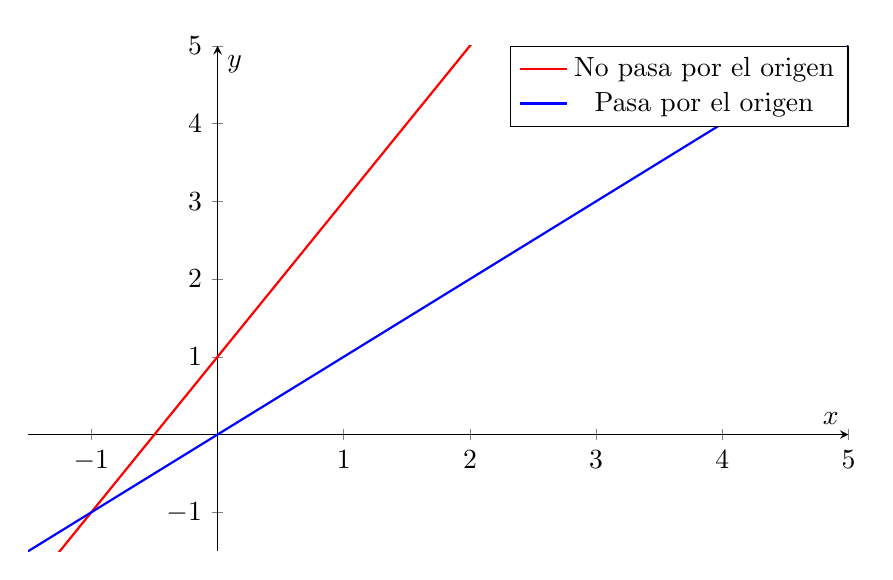
\begin{tikzpicture}
                    \begin{axis}
                        [
                        axis lines=middle,
                        xlabel={$x$},
                        ylabel={$y$},
                        xmin=-1.5, xmax=5,
                        ymin=-1.5, ymax=5,
                        legend style={at={(1,1)}, anchor=north east},
                        width=12cm,
                        height=8cm,
                        ]

                        % Line with positive gradient (y = 2x + 1)
                        \addplot[domain=-5:5, red, thick] {2*x + 1};
                        \addlegendentry{No pasa por el origen}

                        % Line that passes through the origin (y = x)
                        \addplot[domain=-5:5, blue, thick] {x};
                        \addlegendentry{Pasa por el origen}
                    \end{axis}
                \end{tikzpicture}
                \caption{Gráfica de dos magnitudes directamente proporcionales}
            \end{figure}
            \item \negsubro{Inversamente proporcional}
            Son gráficas en forma de curva como \( y = \dfrac{1}{x} \).

            \begin{remark}
                En este tipo de gráfica, si una magnitud aumenta, la otra debe disminuir.
            \end{remark}

            \begin{figure}[H]
                \centering
                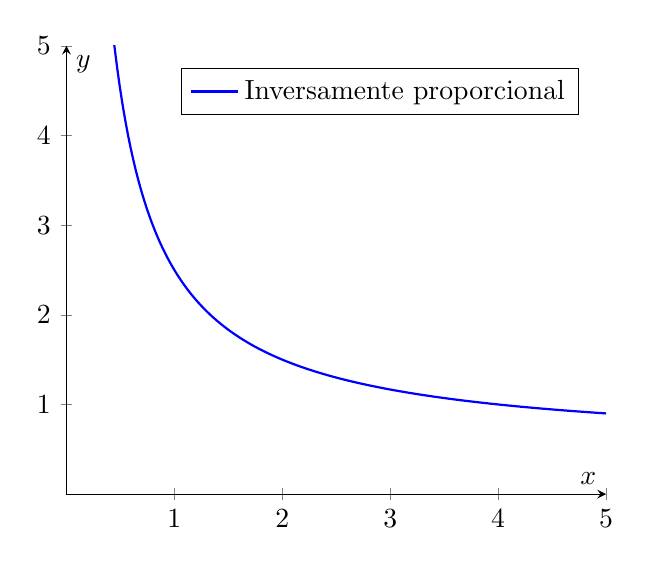
\begin{tikzpicture}
                    \begin{axis}
                        [
                        xlabel={$x$},
                        ylabel={$y$},
                        axis lines=middle,
                        ymin=0, ymax=5,
                        xmin=0, xmax=5,
                        samples=200,
                        domain=0.1:5, % Only the positive side
                        legend style={at={(0.95,0.95)}, anchor=north east},
                        legend entries={Inversamente proporcional}
                        ]
                        \addplot [blue, thick] {0.5 + 2/x};
                    \end{axis}
                \end{tikzpicture}
                \caption{Gráfica de dos magnitudes inversamente proporcionales}
            \end{figure}
        \end{itemize}
\end{enumerate}


\section{Magnitudes Físicas y sus Unidades}

\begin{definition}[Magnitud física]
        Es cualquier propiedad de un cuerpo que podemos medir.
        Por propiedad, entendemos una característica de un objeto.
\end{definition}
\vspace*{-8pt}
A toda magnitud, ya sea física o química, se le asigna una \textbf{unidad}.
\begin{definition}[Unidad]
        Una unidad es una cantidad definida por convenio para establecer un patrón.
\end{definition}
\vspace*{6pt}
Existen varios sistemas de unidades, pero el más utilizado es el Sistema Internacional de Unidades (SI).

Fue creado en 1960 por la Conferencia General de Pesas y Medidas y consta de 7 unidades básicas o fundamentales.

Gracias al sistema SI, se puede garantizar la fiabilidad de las especificaciones de los objetos en el comercio internacional.

Clasificamos las magnitudes en dos tipos:

\begin{itemize}
    \item \textbf{Magnitudes fundamentales}.
    Se definen por sí mismas; son las magnitudes básicas que no pueden descomponerse en otras magnitudes.

    En la Tabla \ref{tab:magnitudes_fundamentales}, se enumeran las magnitudes fundamentales, sus símbolos, las unidades del SI y los símbolos de las unidades.

    % Añade en el preámbulo: \usepackage{makecell}

    \begin{table}[H]
        \centering
        \caption{Magnitudes Fundamentales}
        \vspace{-5pt}
        \begin{tabular}{@{}lccc@{}}
            \toprule
            \textbf{Magnitud} & \makecell{\textbf{Símbolo de} \\ \textbf{la magnitud}}              & \textbf{Unidad}         & \makecell{\textbf{Símbolo de} \\ \textbf{la unidad}}                \\
            \midrule
            Longitud         & l         & metro   & \unit{\m} \\[3pt]
            Masa                & m         & kilogramo   & \unit{\kilo\g} \\[3pt]
            Temperatura    & T         & kelvin   & \unit{\kelvin} \\[3pt]
            Tiempo & t         & segundo     & \unit{\s} \\[3pt]
            Intensidad de corriente eléctrica  & I & amperio  & \unit{\ampere} \\[3pt]
            Cantidad de sustancia  & n & mol  & \unit{\mole} \\[3pt]
            Intensidad luminosa  & \( I_v \) & candela  & \unit{\candela} \\
            \bottomrule
        \end{tabular}
        \label{tab:magnitudes_fundamentales}
    \end{table}

%    \begin{table}[H]
%        \centering
%        \caption{Fundamental quantities}
%        \label{table:fundamental_quantities}
%        \begin{tblr}
%        {
%            colspec={|c|c|c|c|},
%            row{1} = {bg=darkblue!80, fg=white, font=\bfseries},
%            hlines,
%            vlines
%        }
%            Quantity & Quantity Symbol & Unit & Unit Symbol \\
%            Length & l & metre & \unit{\m} \\
%            Mass & m & kilogram & \unit{\kilo\g} \\
%            Temperature & T & kelvin & \unit{\kelvin} \\
%            Time & t & second & \unit{\s} \\
%            Electric current & I & ampere & \unit{\ampere} \\
%            Amount of substance & n & mole & \unit{\mole} \\
%            Luminous intensity & \( I_v \) & candela & \unit{\candela} \\
%        \end{tblr}
%    \end{table}


    \item \textbf{Magnitudes derivadas}.
    Se forman a partir de las magnitudes fundamentales y pueden expresarse como combinaciones de estas.

    La Tabla \ref{tab:derivative_quantities} enumera algunas magnitudes derivadas con sus unidades en el Sistema Internacional.

    \begin{table}[H]
        \centering
        \caption{Magnitudes Derivadas}
        \vspace{-5pt}
        \begin{tabular}{@{}lccc@{}}
            \toprule
            \textbf{Magnitud} & \makecell{\textbf{Símbolo de} \\ \textbf{la magnitud}}     & \textbf{Unidad}          & \makecell{\textbf{Símbolo de} \\ \textbf{la unidad}}   \\
            \midrule
            Área  & A & metro cuadrado           & \unit{\square\m} \\[3pt]
            Volumen    & V          & metro cúbico           & \unit{\cubic\m} \\[3pt]
            Densidad    & \( \rho \)          & --       & \unit{\kilo\g\per\cubic\m} \\[3pt]
            Velocidad & v          & --       & \unit{\mps} \\[3pt]
            Fuerza   & F          & newton        & \unit{\newton} \\[3pt]
            Presión   & p          & pascal        & \unit{\pascal} \\[3pt]
            Energía   & E          & julio        & \unit{\joule} \\[3pt]
            \bottomrule
        \end{tabular}
        \label{tab:derivative_quantities}
    \end{table}

%    \begin{table}[H]
%        \centering
%        \caption{Derivative quantities}
%        \label{table:derivative_quantities}
%        \begin{tblr}{
%            colspec={|c|c|c|c|},
%            row{1} = {bg=darkblue!80, fg=white, font=\bfseries},
%            hlines,
%            vlines
%        }
%            Quantity & Quantity Symbol & Unit & Unit Symbol \\
%            Area & A & square metre & \unit{\square\m} \\
%            Volume & V & cubic metre & \unit{\cubic\m} \\
%            Density & \( \rho \) & -- & \unit{\kilo\g\per\cubic\m} \\
%            Speed & v & -- & \unit{\mps} \\
%            Force & F & newton & \unit{\newton} \\
%            Pressure & p & pascal & \unit{\pascal} \\
%            Energy & E & joule & \unit{\joule} \\
%        \end{tblr}
%    \end{table}
\end{itemize}

\begin{remark}
    Si queremos determinar si una magnitud es fundamental o derivada, el método más sencillo es aprenderse las fundamentales.
    Si no es fundamental, entonces es derivada.
\end{remark}

\begin{exercise}
    En tu cuaderno, indica cuáles de las siguientes magnitudes son fundamentales y cuáles son derivadas:
    \vspace*{-12pt}
    \begin{multicols}{3}
        \begin{enumerate}[label=\letraminuscula]
            \item Intensidad de corriente eléctrica.
            \item Presión.
            \item Velocidad.
            \item Masa.
            \item Temperatura.
            \item Densidad.
            \item Energía.
            \item Longitud.
            \item Cantidad de sustancia
        \end{enumerate}
    \end{multicols}
    \begin{solu}
        En tu cuaderno, indica cuáles de las siguientes magnitudes son fundamentales y cuáles son derivadas:
        \begin{multicols}{2}
            \begin{enumerate}[label=\letraminuscula]
            \item Intensidad de corriente eléctrica. \textcolor{ocre}{Derivada}
            \item Presión. \textcolor{ocre}{Derivada}
            \item Velocidad. \textcolor{ocre}{Derivada}
            \item Masa. \textcolor{ocre}{Fundamental}
            \item Temperatura. \textcolor{ocre}{Fundamental}
            \item Densidad. \textcolor{ocre}{Derivada}
            \item Energía.\textcolor{ocre}{Derivada}
            \item Longitud. \textcolor{ocre}{Fundamental}
            \end{enumerate}
        \end{multicols}
    \end{solu}
\end{exercise}

\subsection{Múltiplos y Submúltiplos}

Al definir un sistema de unidades, también es necesario establecer los múltiplos y submúltiplos de dichas unidades, que nos permiten trabajar con cantidades numéricas más manejables.

La siguiente tabla muestra la relación entre una unidad y los distintos factores de proporcionalidad correspondientes a sus múltiplos y submúltiplos.
\begin{multicols}{2}
    \begin{table}[H]
        \centering
        \caption{Múltiplos}
        \vspace{-5pt}
        \begin{tabular}{@{}ccc@{}}
            \toprule
            \textbf{Orden de Magnitud} & \textbf{Nombre} & \textbf{Símbolo} \\
            \midrule
            \num{e12}                   & tera-         & T     \\[3pt]
            \num{e9}                    & giga-         & G               \\[3pt]
            \num{e6}                    & mega-         & M               \\[3pt]
            \num{e3}                    & kilo-         & k               \\[3pt]
            \num{e2}                    & hecto-        & h               \\[3pt]
            \num{10}                    & deca-         & da              \\[3pt]
            \bottomrule
            \multicolumn{3}{c}{\textbf{Unidad Base} }
            \\
            \bottomrule
        \end{tabular}
        \label{tab:Multiples}
    \end{table}
%    \begin{table}[H]
%        \caption{Multiples}
%        \label{table:Multiples}
%        \begin{tblr}{
%            colspec={|c|c|c|},
%            row{1} = {bg=darkblue!80, fg=white, font=\bfseries},
%            hlines,
%            vlines
%        }
%            Order of Magnitude & Name  & Symbol \\
%            \num{e12} & tera- & T \\
%            \num{e9} & giga- & G \\
%            \num{e6} & mega- & M \\
%            \num{e3} & kilo- & k \\
%            \num{e2} & hecto- & h \\
%            \num{10} & deca- & da \\
%            \SetRow{darkblue!70}\SetCell[c=3]{c} \textbf{\textcolor{white}{Base Unit}}
%        \end{tblr}
%    \end{table}
    \columnbreak
    \begin{table}[H]
        \centering
        \caption{Submúltiplos}
        \vspace{-5pt}
        \begin{tabular}{@{}ccc@{}}
            \toprule
            \textbf{Orden de Magnitud} & \textbf{Nombre} & \textbf{Símbolo} \\
            \toprule
            \multicolumn{3}{c}{\textbf{Unidad Base} } \\
            \toprule
            \num{e-1}                   & deci-         & d \\[3pt]
            \num{e-2}                   & centi-        & c \\[3pt]
            \num{e-3}                   & mili-        & m \\[3pt]
            \num{e-6}                   & micro-        & \( \mu \) \\[3pt]
            \num{e-9}                   & nano-         & n \\[3pt]
            \num{e-12}                  & pico-         & p               \\
            \bottomrule
        \end{tabular}
        \label{tab:Submultiples}
    \end{table}
%    \begin{table}[H]
%        \caption{Submultiples}
%        \label{table:Submultiples}
%
%        \begin{tblr}{
%            colspec={|c|c|c|},
%            row{1} = {bg=darkblue!80, fg=white, font=\bfseries},
%            hlines,
%            vlines
%        }
%            Order of Magnitude & Name  & Symbol \\
%            \SetRow{darkblue!70}\SetCell[c=3]{c} \textbf{\textcolor{white}{Base Unit}} \\
%            \num{e-1} & deci- & d \\
%            \num{e-2} & centi- & c \\
%            \num{e-3} & milli- & m \\
%            \num{e-6} & micro- & \( \mu \) \\
%            \num{e-9} & nano- & n \\
%            \num{e-12} & pico- & p \\
%        \end{tblr}
%    \end{table}
\end{multicols}

Las unidades del SI no son las únicas en uso; de hecho, casi todas las magnitudes tienen varias unidades posibles.
La siguiente tabla muestra magnitudes con distintas unidades y sus equivalencias con otras unidades de la misma magnitud.

\begin{table}[H]
    \centering
    \caption{Magnitudes con sus equivalencias}
    \vspace{-5pt}
    \begin{tabular}{@{}ccc@{}}
        \toprule
        \textbf{Magnitud}         & \textbf{Unidad}                   & \textbf{Equivalencia de la unidad}                           \\
        \midrule
        \multirow{3}{*}{Volumen}   & \unit{\kilo\litre}              & \qty{1}{\kilo\litre} = \qty{1}{\cubic\metre}        \\[3pt]
        & \unit{\litre}                   & \qty{1}{\litre} = \qty{1}{\cubic\deci\metre}        \\[3pt]
        & \unit{\milli\litre}             & \qty{1}{\milli\litre} = \qty{1}{\cubic\centi\metre} \\[3pt]
        \midrule
        \multirow{3}{*}{Presión} & Atmósfera (\unit{\atmosphere}) & \qty{1}{\atmosphere} = \qty{e5}{\pascal} \\[3pt]
        & \makecell{milímetro de mercurio \\  (\unit{\mmHg})}                    & \qty{1}{\atmosphere} = \qty{760}{\mmHg} \\[3pt]
        \midrule
        Energía                     & Caloría (\unit{\cal})           & \qty{1}{\cal} = \qty{4.18}{\joule}                   \\[3pt]
        \midrule
        Fuerza                     & Kilopondio (\unit{\kp})           & \qty{1}{\kp} = \qty{9.8}{\newton}                   \\
        \bottomrule
    \end{tabular}
    \label{tab:quantities_with_their_equivalences}
\end{table}

%\begin{table}[H]
%    \centering
%    \caption{Quantities with their equivalences}
%    \label{table:quantities_with_their_equivalences}
%    \begin{tblr}{
%        colspec={|c|c|c|},
%        row{1} = {bg=darkblue!80, fg=white, font=\bfseries},
%        hlines,
%        vlines,
%        cell{2}{1}={r=3}{c},
%        cell{5}{1}={r=2}{c},
%        rowhead=1
%    }
%        Quantity & Unit & Unit Equivalence \\
%        Volume & \unit{\kilo\litre} & \qty{1}{\kilo\litre} = \qty{1}{\cubic\metre} \\
%        & \unit{\litre} & \qty{1}{\litre} = \qty{1}{\cubic\deci\metre} \\
%        & \unit{\milli\litre} & \qty{1}{\milli\litre} = \qty{1}{\cubic\centi\metre} \\
%        Pressure & {Atmosphere \\ (\unit{\atmosphere})} & \qty{1}{\atmosphere} = \qty{e5}{\pascal} \\
%        & {millimetre of mercury \\ (\unit{\mmHg})} & \qty{1}{\atmosphere} = \qty{760}{\mmHg} \\
%        Energy & Calorie (\unit{\cal}) & \qty{1}{\cal} = \qty{4.18}{\joule} \\
%        Force & Kilopond (\unit{\kp}) & \qty{1}{\kp} = \qty{9.8}{\newton} \\
%    \end{tblr}
%\end{table}

\subsection{Conversión de Unidades Mediante Factores de Conversión}

Primero debemos tener en cuenta lo siguiente:
\begin{enumerate}[label=\letraminuscula]
        \item Podemos convertir entre unidades siempre que pertenezcan a la misma magnitud.
        \item Podemos convertir entre unidades con distintos múltiplos y submúltiplos.
        \item También podemos convertir entre distintas unidades siempre que representen la misma magnitud y conozcamos la equivalencia entre ellas.
\end{enumerate}

\begin{example}
    Convirtamos \qty{36}{\kmph} a \unit{\mps}:
    \begin{equation*}
        36\ \dfrac{\cancelred{\unit{\kilo\metre}}}{\cancel{\unit{\hour}}} \cdot \dfrac{1000\ \unit{\metre}}{1\ \cancelred{\unit{\kilo\metre}}} \cdot \dfrac{1\ \cancelred{\unit{\hour}}}{3600\ \unit{\second}} = \dfrac{36 \cdot 1000}{3600} = \qty{10}{\mps}
    \end{equation*}
\end{example}

\begin{example}
    Convierte \qty{13600}{\kilo\g\per\cubic\metre} a \unit{\g\per\cubic\centi\metre}:
    \begin{equation*}
        13600\ \dfrac{\cancelred{\unit{\kilo\g}}}{\cancel{\unit{\cubic\metre}}} \cdot \dfrac{1000\ \unit{\g}}{1\ \cancelred{\unit{\kilo\g}}} \cdot \dfrac{1\ \cancelred{\unit{\cubic\metre}}}{\num{e6}\ \unit{\cubic\centi\metre}} = \dfrac{13600 \cdot 1000}{\num{e6}} = \qty{13.6}{\g\per\cubic\centi\metre}
    \end{equation*}
\end{example}

\begin{example}
    Convierte \qty{12}{\kilo\metre} a \unit{\nano\metre}:
    \begin{equation*}
        12\ \cancelred{\unit{\kilo\metre}} \cdot  \dfrac{\num{e12}\ \unit{\nano\metre}}{ 1\ \cancelred{\unit{\kilo\metre}}} = \num{12e-12} = \qty{1.2e-11}{\nano\metre}
    \end{equation*}
\end{example}

\begin{exercise}
    Convierte las siguientes velocidades a las unidades indicadas utilizando factores de conversión.
    \begin{enumerate}[label=\letraminuscula]
        \item Convierte las siguientes velocidades a \unit{\mps}:
        \begin{multicols}{4}
            \begin{itemize}
                \item \qty{90}{\kmph}
                \item \qty{100}{\kmph}
                \item \qty{120}{\kmph}
                \item \qty{50}{\kmph}
            \end{itemize}
        \end{multicols}
        \item Convierte las siguientes velocidades a \unit{\kmph}:
        \begin{multicols}{4}
            \begin{itemize}
                \item \qty{12}{\mps}
                \item \qty{340}{\mps}
                \item \qty{0.36}{\mps}
                \item \qty{3e8}{\mps}
            \end{itemize}
        \end{multicols}
    \end{enumerate}
    \begin{solu}

        Para realizar estas conversiones, utilizamos las siguientes relaciones de equivalencia: $1 \text{ km} = 1000 \text{ m}$ y $1 \text{ h} = 3600 \text{ s}$.

        \textbf{a) Conversión de km/h a m/s:}
        \begin{itemize}
            \item \textbf{90 km/h}:
            \[ 90 \frac{\cancel{\text{km}}}{\cancel{\text{h}}} \cdot \frac{1000 \text{ m}}{1 \cancel{\text{km}}} \cdot \frac{1 \cancel{\text{h}}}{3600 \text{ s}} = \frac{90 \cdot 1000}{3600} \text{ m/s} = 25 \text{ m/s} \]

            \item \textbf{100 km/h}:
            \[ 100 \frac{\cancel{\text{km}}}{\cancel{\text{h}}} \cdot \frac{1000 \text{ m}}{1 \cancel{\text{km}}} \cdot \frac{1 \cancel{\text{h}}}{3600 \text{ s}} = \frac{100000}{3600} \text{ m/s} \approx 27.78 \text{ m/s} \]

            \item \textbf{120 km/h}:
            \[ 120 \frac{\cancel{\text{km}}}{\cancel{\text{h}}} \cdot \frac{1000 \text{ m}}{1 \cancel{\text{km}}} \cdot \frac{1 \cancel{\text{h}}}{3600 \text{ s}} = \frac{120000}{3600} \text{ m/s} \approx 33.33 \text{ m/s} \]

            \item \textbf{50 km/h}:
            \[ 50 \frac{\cancel{\text{km}}}{\cancel{\text{h}}} \cdot \frac{1000 \text{ m}}{1 \cancel{\text{km}}} \cdot \frac{1 \cancel{\text{h}}}{3600 \text{ s}} = \frac{50000}{3600} \text{ m/s} \approx 13.89 \text{ m/s} \]
        \end{itemize}

        \textbf{b) Conversión de m/s a km/h:}
        \begin{itemize}
            \item \textbf{12 m/s}:
            \[ 12 \frac{\cancel{\text{m}}}{\cancel{\text{s}}} \cdot \frac{1 \text{ km}}{1000 \cancel{\text{m}}} \cdot \frac{3600 \cancel{\text{s}}}{1 \text{ h}} = 12 \cdot 3.6 \text{ km/h} = 43.2 \text{ km/h} \]

            \item \textbf{340 m/s}:
            \[ 340 \frac{\cancel{\text{m}}}{\cancel{\text{s}}} \cdot \frac{1 \text{ km}}{1000 \cancel{\text{m}}} \cdot \frac{3600 \cancel{\text{s}}}{1 \text{ h}} = 340 \cdot 3.6 \text{ km/h} = 1224 \text{ km/h} \]

            \item \textbf{0.36 m/s}:
            \[ 0.36 \frac{\cancel{\text{m}}}{\cancel{\text{s}}} \cdot \frac{1 \text{ km}}{1000 \cancel{\text{m}}} \cdot \frac{3600 \cancel{\text{s}}}{1 \text{ h}} = 0.36 \cdot 3.6 \text{ km/h} = 1.296 \text{ km/h} \]

            \item \textbf{$3 \cdot 10^8$ m/s}:
            \[ 3 \cdot 10^8 \frac{\cancel{\text{m}}}{\cancel{\text{s}}} \cdot \frac{1 \text{ km}}{1000 \cancel{\text{m}}} \cdot \frac{3600 \cancel{\text{s}}}{1 \text{ h}} = 3 \cdot 10^8 \cdot 3.6 \text{ km/h} = 1.08 \cdot 10^9 \text{ km/h} \]
        \end{itemize}
    \end{solu}
\end{exercise}


\begin{exercise}
    Convierte las siguientes unidades a las unidades del SI correspondientes utilizando factores de conversión.
    \begin{multicols}{4}
        \begin{enumerate}[label=\letraminuscula]
            \item \qty{200}{\square\centi\metre}
            \item \qty{125}{\cubic\centi\metre}
            \item \qty{1800}{\g}
            \item \qty{45}{\min}
        \end{enumerate}
    \end{multicols}


    \begin{solu}
        Para convertir estos valores al Sistema Internacional de Unidades (SI), utilizamos las unidades básicas: metros (\unit{\m}), kilogramos (\unit{\kg}) y segundos (\unit{\s}).

        \textbf{a) Conversión de área (\unit{\square\centi\metre} a \unit{\square\metre}):}
        Dado que \( \qty{1}{\metre} = \qty{100}{\centi\metre} \), entonces \( \qty{1}{\square\metre} = (\qty{100}{\centi\metre})^2 = \qty{10000}{\square\centi\metre} \).
        \[ \qty{200}{\cancel{\square\centi\metre}} \cdot \frac{\qty{1}{\square\metre}}{\qty{10000}{\cancel{\square\centi\metre}}} = \qty{0.02}{\square\metre} \]

        \textbf{b) Conversión de volumen (\unit{\cubic\centi\metre} a \unit{\cubic\metre}):}
        Dado que \( \qty{1}{\metre} = \qty{100}{\centi\metre} \), entonces \( \qty{1}{\cubic\metre} = (\qty{100}{\centi\metre})^3 = \qty{1000000}{\cubic\centi\metre} \).
        \[ \qty{125}{\cancel{\cubic\centi\metre}} \cdot \frac{\qty{1}{\cubic\metre}}{\qty{1000000}{\cancel{\cubic\centi\metre}}} = \qty{1.25e-4}{\cubic\metre} \]

        \textbf{c) Conversión de masa (\unit{\g} a \unit{\kg}):}
        Equivalencia: \( \qty{1}{\kg} = \qty{1000}{\g} \).
        \[ \qty{1800}{\cancel{\g}} \cdot \frac{\qty{1}{\kg}}{\qty{1000}{\cancel{\g}}} = \qty{1.8}{\kg} \]

        \textbf{d) Conversión de tiempo (\unit{\min} a \unit{\s}):}
        Equivalencia: \( \qty{1}{\min} = \qty{60}{\s} \).
        \[ \qty{45}{\cancel{\min}} \cdot \frac{\qty{60}{\s}}{\qty{1}{\cancel{\min}}} = \qty{2700}{\s} \]
    \end{solu}

\end{exercise}

\begin{exercise}
    Realiza las siguientes conversiones de unidades a unidades del SI utilizando factores de conversión
    \begin{multicols}{4}
        \begin{enumerate}[label=\letraminuscula]
\item \qty{300}{\mmHg}
\item \qty{25000}{\cal}
\item \qty{21}{\atmosphere}
\item \qty{258}{\kilopondio}
        \end{enumerate}
    \end{multicols}


    \begin{solu}
        En el Sistema Internacional, la unidad derivada de la presión es el Pascal (\unit{\Pa}), la de la energía es el Julio (\unit{\J}) y la de la fuerza es el Newton (\unit{\N}).

        \textbf{a) Presión (\unit{\mmHg} a \unit{\Pa}):}
        Equivalencia: \( \qty{760}{\mmHg} = \qty{101325}{\Pa} \).
        \[ \qty{300}{\cancel{\mmHg}} \cdot \frac{\qty{101325}{\Pa}}{\qty{760}{\cancel{\mmHg}}} \approx \qty{39996.71}{\Pa} \]

        \textbf{b) Energía (\unit{cal} a \unit{\J}):}
        Equivalencia: \( \qty{1}{cal} = \qty{4.184}{\J} \).
        \[ \qty{25000}{\cancel{cal}} \cdot \frac{\qty{4.184}{\J}}{\qty{1}{\cancel{cal}}} = \qty{104600}{\J} \]

        \textbf{c) Presión (\unit{atm} a \unit{\Pa}):}
        Equivalencia: \( \qty{1}{atm} = \qty{101325}{\Pa} \).
        \[ \qty{21}{\cancel{atm}} \cdot \frac{\qty{101325}{\Pa}}{\qty{1}{\cancel{atm}}} = \qty{2127825}{\Pa} \]

        \textbf{d) Fuerza (\unit{kp} a \unit{\N}):}
        Equivalencia: \( \qty{1}{kp} = \qty{9.8}{\N} \).
        \[ \qty{258}{\cancel{kp}} \cdot \frac{\qty{9.8}{\N}}{\qty{1}{\cancel{kp}}} = \qty{2528.4}{\N} \]
    \end{solu}

\end{exercise}

\begin{exercise}
    Si 1 g de oro puro cuesta 31,32 €, calcula el precio de 1 dg y 1 cg de este metal. Resuelve el siguiente ejercicio utilizando factores de conversión.

    \begin{solu}
        Usando las relaciones de masa dentro del sistema decimal: \( \qty{1}{\g} = \qty{10}{\deci\g} \) y \( \qty{1}{\g} = \qty{100}{\centi\g} \).

        \textbf{1) Precio de \qty{1}{\deci\g}:}
        \[ \qty{1}{\cancel{\deci\g}} \cdot \frac{\qty{1}{\cancel{\g}}}{\qty{10}{\cancel{\deci\g}}} \cdot \frac{\text{31.32 €}}{\qty{1}{\cancel{\g}}} = \text{3.13 €} \]

        \textbf{2) Precio de \qty{1}{\centi\g}:}
        \[ \qty{1}{\cancel{\centi\g}} \cdot \frac{\qty{1}{\cancel{\g}}}{\qty{100}{\cancel{\centi\g}}} \cdot \frac{\text{31.32 €}}{\qty{1}{\cancel{\g}}} = \text{0.31 €} \]
    \end{solu}

\end{exercise}

\begin{exercise}
    Si 1 kg de almendras cuesta 18,40 €, calcula el precio de 1 hg y 1 dag de este producto. Resuelve el siguiente ejercicio utilizando factores de conversión.

    \begin{solu}
        Usando las relaciones de masa dentro del sistema decimal: \( \qty{1}{\kg} = \qty{10}{\hecto\g} \) y \( \qty{1}{\kg} = \qty{100}{\deca\g} \).

        \textbf{1) Precio de \qty{1}{\hecto\g}:}
        \[
        \qty{1}{\cancel{\hecto\g}} \cdot
        \frac{\qty{1}{\cancel{\kg}}}{\qty{10}{\cancel{\hecto\g}}} \cdot
        \frac{\text{18.40 €}}{\qty{1}{\cancel{\kg}}}
        = \text{1.84 €}
        \]

        \textbf{2) Precio de \qty{1}{\deca\g}:}
        \[
        \qty{1}{\cancel{\deca\g}} \cdot
        \frac{\qty{1}{\cancel{\kg}}}{\qty{100}{\cancel{\deca\g}}} \cdot
        \frac{\text{18.40 €}}{\qty{1}{\cancel{\kg}}}
        = \text{0.184 €}
        \]
    \end{solu}

\end{exercise}

\begin{exercise}
    Si 1 L de aceite de oliva cuesta 9,60 €, calcula el precio de 1 dL y 1 cL de este líquido. Resuelve el siguiente ejercicio utilizando factores de conversión.

    \begin{solu}
        Usando las relaciones de capacidad dentro del sistema decimal: \( \qty{1}{\L} = \qty{10}{\deci\L} \) y \( \qty{1}{\L} = \qty{100}{\centi\L} \).

        \textbf{1) Precio de \qty{1}{\deci\L}:}
        \[
        \qty{1}{\cancel{\deci\L}} \cdot
        \frac{\qty{1}{\cancel{\L}}}{\qty{10}{\cancel{\deci\L}}} \cdot
        \frac{\text{9.60 €}}{\qty{1}{\cancel{\L}}}
        = \text{0.96 €}
        \]

        \textbf{2) Precio de \qty{1}{\centi\L}:}
        \[
        \qty{1}{\cancel{\centi\L}} \cdot
        \frac{\qty{1}{\cancel{\L}}}{\qty{100}{\cancel{\centi\L}}} \cdot
        \frac{\text{9.60 €}}{\qty{1}{\cancel{\L}}}
        = \text{0.096 €}
        \]
    \end{solu}

\end{exercise}


\section{Notación Científica}

La notación científica nos permite escribir números muy grandes o muy pequeños utilizando potencias de \num{10}, con un exponente positivo para números muy grandes o un exponente negativo para números muy pequeños.

Para que un número esté correctamente expresado en notación científica, debe tener:

\begin{itemize}
    \item Un único dígito distinto de cero a la izquierda de la coma decimal.
    \item Una potencia de 10 elevada a un exponente positivo o negativo.
\end{itemize}

Por ejemplo:

\begin{itemize}
    \item La masa de la Tierra es:

    \qty{6000000000000000000000000}{\kilo\g}.
    Como podemos ver, este número tiene 24 ceros, por lo que escribirlo repetidamente resulta bastante tedioso.
    Este número en notación científica sería: \qty{6e24}{\kilo\g}.

    \item La masa del electrón es:

    \qty{0.0000000000000000000000000000009109}{\kilo\g}.
    Este número en notación científica se escribe como \qty{9.3109e-31}{\kilo\g}.
\end{itemize}

Los pasos para convertir a notación científica son los siguientes:

\begin{itemize}
    \item \textbf{Números mayores que uno}.
    Comenzamos por la derecha del número.
    En ese punto, colocamos la coma decimal y contamos cuántas posiciones necesitamos desplazarla para que quede un único dígito distinto de cero a su izquierda.
    El número en notación científica será el nuevo número multiplicado por una potencia de 10, elevada al número de posiciones desplazadas, con exponente positivo.
    Por eso, en el caso anterior obtenemos \num{6e24}.

    \item \textbf{Números menores que uno}.
    Comenzamos por la coma decimal y contamos cuántas posiciones necesitamos desplazarla para que quede un único dígito distinto de cero a su izquierda.
    El exponente resultante será negativo.

    \item \textbf{Números que ya son grandes o pequeños pero que ya incluyen una potencia de 10} .
    Comenzamos por la coma decimal.
    Pueden darse los siguientes casos:

    \begin{itemize}
        \item Si el número es mayor que uno:
        Procedemos como en el caso anterior, y el número de posiciones se \emph{suma} al exponente de la potencia decimal. Ejemplos:
        \begin{itemize}
            \item \num{625.5e5} se convierte en \num{6.255e7}.
            \item \num{45654.21e-2} se convierte en \num{4.5654e-2}.
        \end{itemize}

        \item Si el número es menor que uno:
        Procedemos de forma similar, pero en este caso el número de posiciones se \emph{resta} del exponente. Ejemplos:
        \begin{itemize}
            \item \num{0.0523e-3} se convierte en \num{5.23e-5}.
            \item \num{0.000254e5} se convierte en \num{2.54e-1}.
        \end{itemize}
    \end{itemize}
\end{itemize}

\begin{exercise}
    Escribe las siguientes cantidades en notación científica:
    \begin{multicols}{3}
        \begin{enumerate}[label=\letraminuscula]
\item \qty{20000000}{\m}
\item \qty{250000000}{\litre}
\item \qty{7820000000}{\g}
\item \qty{254830368}{\km}
\item \qty{0.0001}{\s}
\item \qty{0.000035}{\kilo\g}
\item \qty{0.000001}{\m}
\item \qty{0.000005001}{\g}
\item \qty{0.000000005}{\g}
        \end{enumerate}
    \end{multicols}

    \begin{solu}
        Para escribir en notación científica, desplazamos la coma decimal para obtener un número entre 1 y 10, y luego multiplicamos por la potencia de 10 correspondiente.
        \begin{itemize}
            \item \textbf{a)} \( \qty{20000000}{\m} = \qty{2e7}{\m} \)
            \item \textbf{b)} \( \qty{250000000}{\litre} = \qty{2.5e8}{\litre} \)
            \item \textbf{c)} \( \qty{7820000000}{\g} = \qty{7.82e9}{\g} \)
            \item \textbf{d)} \( \qty{254830368}{\km} \approx \qty{2.55e8}{\km} \)
            \item \textbf{e)} \( \qty{0.0001}{\s} = \qty{1e-4}{\s} \)
            \item \textbf{f)} \( \qty{0.000035}{\kg} = \qty{3.5e-5}{\kg} \)
            \item \textbf{g)} \( \qty{0.000001}{\m} = \qty{1e-6}{\m} \)
            \item \textbf{h)} \( \qty{0.000005001}{\g} = \qty{5.001e-6}{\g} \)
            \item \textbf{i)} \( \qty{0.000000005}{\g} = \qty{5e-9}{\g} \)
        \end{itemize}
    \end{solu}

\end{exercise}
\begin{exercise}
    Escribe las siguientes cantidades en notación científica.
    \begin{multicols}{3}
        \begin{enumerate}[label=\letraminuscula]
\item \qty{0.00005}{\g}
\item \qty{0.000052}{\g}
\item \qty{2000000}{\m}
\item \qty{25000000}{\m}
\item \qty{301000}{\s}
\item \qty{0.000205}{\ampere}
\item \qty{20520000000}{\kg}
\item \qty{5000000000}{\kg}
        \end{enumerate}
    \end{multicols}

    \begin{solu}
        \begin{itemize}
            \item \textbf{a)} \( \qty{0.00005}{\g} = \qty{5e-5}{\g} \)
            \item \textbf{b)} \( \qty{0.000052}{\g} = \qty{5.2e-5}{\g} \)
            \item \textbf{c)} \( \qty{2000000}{\m} = \qty{2e6}{\m} \)
            \item \textbf{d)} \( \qty{25000000}{\m} = \qty{2.5e7}{\m} \)
            \item \textbf{e)} \( \qty{301000}{\s} = \qty{3.01e5}{\s} \)
            \item \textbf{f)} \( \qty{0.000205}{\ampere} = \qty{2.05e-4}{\ampere} \)
            \item \textbf{g)} \( \qty{20520000000}{\kg} = \qty{2.052e10}{\kg} \)
            \item \textbf{h)} \( \qty{5000000000}{\kg} = \qty{5e9}{\kg} \)
        \end{itemize}
    \end{solu}

\end{exercise}

\begin{exercise}
    Expresa las siguientes medidas en unidades del SI utilizando factores de conversión y notación científica.
    \begin{multicols}{4}
        \begin{enumerate}[label=\letraminuscula]
\item \qty{0.5}{\g}
\item \qty{0.5}{\cubic\centi\metre}
\item \qty{200}{\square\kilo\metre}
\item \qty{2}{\g\per\cubic\centi\metre}
\item \qty{76}{\hecto\m}
\item \qty{3}{\milli\g}
\item \qty{9}{\deca\m}
\item \qty{25}{\nano\s}
        \end{enumerate}
    \end{multicols}

    \begin{solu}
        \begin{itemize}
            \item \textbf{a) \qty{0.5}{\g} a \unit{\kg}:}
            \[ \qty{0.5}{\cancel{\g}} \cdot \frac{\qty{1}{\kg}}{\qty{1000}{\cancel{\g}}} = \qty{5e-4}{\kg} \]
            \item \textbf{b) \qty{0.5}{\cubic\centi\metre} a \unit{\cubic\metre}:}
            \[ \qty{0.5}{\cancel{\cubic\centi\metre}} \cdot \frac{\qty{1}{\cubic\metre}}{\qty{1e6}{\cancel{\cubic\centi\metre}}} = \qty{5e-7}{\cubic\metre} \]
            \item \textbf{c) \qty{200}{\square\kilo\metre} a \unit{\square\metre}:}
            \[ \qty{200}{\cancel{\square\kilo\metre}} \cdot \frac{\qty{1e6}{\square\metre}}{\qty{1}{\cancel{\square\kilo\metre}}} = \qty{2e8}{\square\metre} \]
            \item \textbf{d) \qty{2}{\g\per\cubic\centi\metre} a \unit{\kg\per\cubic\metre}:}
            \[ \frac{\qty{2}{\cancel{\g}}}{\qty{1}{\cancel{\cubic\centi\metre}}} \cdot \frac{\qty{1}{\kg}}{\qty{1000}{\cancel{\g}}} \cdot \frac{\qty{1e6}{\cancel{\cubic\centi\metre}}}{\qty{1}{\cubic\metre}} = \qty{2e3}{\kg\per\cubic\metre} \]
            \item \textbf{e) \qty{76}{\hecto\m} a \unit{\m}:}
            \[ \qty{76}{\cancel{\hecto\m}} \cdot \frac{\qty{100}{\m}}{\qty{1}{\cancel{\hecto\m}}} = \qty{7.6e3}{\m} \]
            \item \textbf{f) \qty{3}{\milli\g} a \unit{\kg}:}
            \[ \qty{3}{\cancel{\milli\g}} \cdot \frac{\qty{1}{\kg}}{\qty{1e6}{\cancel{\milli\g}}} = \qty{3e-6}{\kg} \]
            \item \textbf{g) \qty{9}{\deca\m} a \unit{\m}:}
            \[ \qty{9}{\cancel{\deca\m}} \cdot \frac{\qty{10}{\m}}{\qty{1}{\cancel{\deca\m}}} = \qty{9e1}{\m} \]
            \item \textbf{h) \qty{25}{\nano\s} a \unit{\s}:}
            \[ \qty{25}{\cancel{\nano\s}} \cdot \frac{\qty{1}{\s}}{\qty{1e9}{\cancel{\nano\s}}} = \qty{2.5e-8}{\s} \]
        \end{itemize}
    \end{solu}

\end{exercise}

\begin{exercise}
    Expresa los siguientes volúmenes en unidades del SI utilizando factores de conversión y notación científica:
    \begin{multicols}{4}
        \begin{enumerate}[label=\letraminuscula]
\item \qty{0.5}{\mL}
\item \qty{0.001}{\mL}
\item \qty{33.3}{\kL}
\item \qty{10000}{\litre}
        \end{enumerate}
    \end{multicols}


    \begin{solu}
        Recuerda que, para el volumen, el \unit{\cubic\metre} es la unidad del SI y \( \qty{1}{\litre} = \qty{1}{\cubic\deci\metre} \). Por lo tanto, \( \qty{1000}{\litre} = \qty{1}{\cubic\metre} \).
        \begin{itemize}
            \item \textbf{a) \qty{0.5}{\mL} a \unit{\cubic\metre}:}
            \[ \qty{0.5}{\cancel{\mL}} \cdot \frac{\qty{1}{\cancel{\litre}}}{\qty{1000}{\cancel{\mL}}} \cdot \frac{\qty{1}{\cubic\metre}}{\qty{1000}{\cancel{\litre}}} = \qty{5e-7}{\cubic\metre} \]
            \item \textbf{b) \qty{0.001}{\mL} a \unit{\cubic\metre}:}
            \[ \qty{0.001}{\cancel{\mL}} \cdot \frac{\qty{1}{\cancel{\litre}}}{\qty{1000}{\cancel{\mL}}} \cdot \frac{\qty{1}{\cubic\metre}}{\qty{1000}{\cancel{\litre}}} = \qty{1e-9}{\cubic\metre} \]
            \item \textbf{c) \qty{33.3}{\kL} a \unit{\cubic\metre}:}
            \[ \qty{33.3}{\cancel{\kL}} \cdot \frac{\qty{1000}{\cancel{\litre}}}{\qty{1}{\cancel{\kL}}} \cdot \frac{\qty{1}{\cubic\metre}}{\qty{1000}{\cancel{\litre}}} = \qty{3.33e1}{\cubic\metre} \]
            \item \textbf{d) \qty{10000}{\litre} a \unit{\cubic\metre}:}
            \[ \qty{10000}{\cancel{\litre}} \cdot \frac{\qty{1}{\cubic\metre}}{\qty{1000}{\cancel{\litre}}} = \qty{1e1}{\cubic\metre} \]
        \end{itemize}
    \end{solu}

\end{exercise}

\begin{exercise}
    Elabora un mapa conceptual de la unidad.

    \begin{solu}
        Un mapa conceptual para "Unidades y Medidas" debería incluir:
        \begin{itemize}
            \item \textbf{Magnitudes físicas:} Fundamentales (masa, longitud, tiempo) y Derivadas (velocidad, densidad, volumen).
            \item \textbf{Sistema Internacional (SI):} Unidades estándar como \unit{\kg}, \unit{\m}, \unit{\s}.
            \item \textbf{Instrumentos de medida:} Precisión, exactitud y sensibilidad.
            \item \textbf{Notación científica:} Expresar números muy grandes o muy pequeños mediante potencias de 10.
            \item \textbf{Conversión de unidades:} Uso de factores de conversión y el sistema métrico (prefijos como kilo-, centi-, mili-).
        \end{itemize}
    \end{solu}

\end{exercise}


%\section{Vocabulario}
%
%\begin{vocabulary}[Scientific Method]
%A systematic approach used by scientists to investigate phenomena, acquire new knowledge, or correct and integrate previous knowledge. It involves observation, hypothesis formulation, experimentation, and analysis of results to develop laws, theories, or models. \newline
%\textbf{Translation to Spanish}: Método científico \newline
%% Line 5
%\end{vocabulary}
%
%\begin{vocabulary}[Observation]
%The first stage of the scientific method that involves carefully watching and recording phenomena or events in nature using the senses or instruments. \newline
%\textbf{Translation to Spanish}: Observación \newline
%% Line 9
%\end{vocabulary}
%
%\begin{vocabulary}[Hypothesis]
%A provisional assumption or proposed explanation made to explain a specific fact or phenomenon that can be tested through experimentation. \newline
%\textbf{Translation to Spanish}: Hipótesis \newline
%% Line 15
%\end{vocabulary}
%
%\begin{vocabulary}[Experimentation]
%The process of carrying out controlled experimental tests to verify or refute a hypothesis through systematic observation and measurement. \newline
%\textbf{Translation to Spanish}: Experimentación \newline
%% Line 16
%\end{vocabulary}
%
%\begin{vocabulary}[Law]
%A statement based on repeated experimental observations that describes some aspect of nature, always occurring under the same conditions. Laws are often expressed mathematically. \newline
%\textbf{Translation to Spanish}: Ley \newline
%% Line 21
%\end{vocabulary}
%
%\begin{vocabulary}[Theory]
%A well-substantiated explanation of some aspect of the natural world that is based on a body of facts that have been repeatedly confirmed through observation and experimentation. \newline
%\textbf{Translation to Spanish}: Teoría \newline
%% Line 21
%\end{vocabulary}
%
%\begin{vocabulary}[Model]
%A simplified representation of a system or phenomenon that helps explain and predict its behavior, often using mathematical equations, diagrams, or physical constructs. \newline
%\textbf{Translation to Spanish}: Modelo \newline
%% Line 21
%\end{vocabulary}
%
%\begin{vocabulary}[Variable]
%Any factor, trait, or condition that can exist in differing amounts or types in an experiment or observation. \newline
%\textbf{Translation to Spanish}: Variable \newline
%% Line 33
%\end{vocabulary}
%
%\begin{vocabulary}[Independent Variable]
%The variable that is deliberately changed or controlled in an experiment to test its effects on the dependent variable. It is plotted on the horizontal axis (X-axis). \newline
%\textbf{Translation to Spanish}: Variable independiente \newline
%% Line 35
%\end{vocabulary}
%
%\begin{vocabulary}[Dependent Variable]
%The variable that is measured or observed in an experiment. It depends on the independent variable and is plotted on the vertical axis (Y-axis). \newline
%\textbf{Translation to Spanish}: Variable dependiente \newline
%% Line 36
%\end{vocabulary}
%
%\begin{vocabulary}[Directly Proportional]
%A relationship between two quantities where if one quantity increases, the other also increases at a constant rate. Graphically represented by a straight line with equation y = mx + n. \newline
%\textbf{Translation to Spanish}: Directamente proporcional \newline
%% Line 61
%\end{vocabulary}
%
%\begin{vocabulary}[Inversely Proportional]
%A relationship between two quantities where if one quantity increases, the other decreases. Graphically represented by a hyperbolic curve of the form y = 1/x. \newline
%\textbf{Translation to Spanish}: Inversamente proporcional \newline
%% Line 96
%\end{vocabulary}
%
%\begin{vocabulary}[Gradient]
%The slope of a line in a graph, represented by the letter m in the equation y = mx + n. It indicates the rate of change of the dependent variable with respect to the independent variable. \newline
%\textbf{Translation to Spanish}: Pendiente \newline
%% Line 64
%\end{vocabulary}
%
%\begin{vocabulary}[Physical Quantity]
%Any property of a body or system that can be measured and expressed numerically with an appropriate unit. \newline
%\textbf{Translation to Spanish}: Magnitud física \newline
%% Line 129
%\end{vocabulary}
%
%\begin{vocabulary}[Unit]
%A quantity defined by convention to establish a standard for measurement. It provides a reference to express the value of physical quantities. \newline
%\textbf{Translation to Spanish}: Unidad \newline
%% Line 135
%\end{vocabulary}
%
%\begin{vocabulary}[International System of Units (SI)]
%The modern form of the metric system established in 1960 by the General Conference on Weights and Measures, consisting of 7 base units and derived units for measuring physical quantities. \newline
%\textbf{Translation to Spanish}: Sistema Internacional de Unidades \newline
%% Line 138
%\end{vocabulary}
%
%\begin{vocabulary}[Fundamental Quantities]
%Basic physical quantities that cannot be broken down into other quantities and are defined independently. Examples include length, mass, time, temperature, electric current, amount of substance, and luminous intensity. \newline
%\textbf{Translation to Spanish}: Magnitudes fundamentales \newline
%% Line 147
%\end{vocabulary}
%
%\begin{vocabulary}[Derived Quantities]
%Physical quantities that are defined in terms of combinations of fundamental quantities. Examples include area, volume, velocity, and density. \newline
%\textbf{Translation to Spanish}: Magnitudes derivadas \newline
%% Line 195 (approximately, based on context)
%\end{vocabulary}
%
%\begin{vocabulary}[Length]
%A fundamental quantity that measures the distance between two points. The SI unit is the metre (m). \newline
%\textbf{Translation to Spanish}: Longitud \newline
%% Line 162
%\end{vocabulary}
%
%\begin{vocabulary}[Mass]
%A fundamental quantity that measures the amount of matter in an object. The SI unit is the kilogram (kg). \newline
%\textbf{Translation to Spanish}: Masa \newline
%% Line 163
%\end{vocabulary}
%
%\begin{vocabulary}[Temperature]
%A fundamental quantity that measures the degree of hotness or coldness of a body. The SI unit is the kelvin (K). \newline
%\textbf{Translation to Spanish}: Temperatura \newline
%% Line 164
%\end{vocabulary}
%
%\begin{vocabulary}[Time]
%A fundamental quantity that measures the duration of events or the interval between them. The SI unit is the second (s). \newline
%\textbf{Translation to Spanish}: Tiempo \newline
%% Line 165
%\end{vocabulary}
%
%\begin{vocabulary}[Electric Current]
%A fundamental quantity that measures the flow of electric charge through a conductor. The SI unit is the ampere (A). \newline
%\textbf{Translation to Spanish}: Corriente eléctrica \newline
%% Line 166
%\end{vocabulary}
%
%\begin{vocabulary}[Amount of Substance]
%A fundamental quantity that measures the number of elementary entities (atoms, molecules, ions, etc.) in a sample. The SI unit is the mole (mol). \newline
%\textbf{Translation to Spanish}: Cantidad de sustancia \newline
%% Line 167
%\end{vocabulary}
%
%\begin{vocabulary}[Luminous Intensity]
%A fundamental quantity that measures the power emitted by a light source in a particular direction. The SI unit is the candela (cd). \newline
%\textbf{Translation to Spanish}: Intensidad luminosa \newline
%% Line 168
%\end{vocabulary}
%
%\begin{vocabulary}[Scientific Notation]
%A method of writing very large or very small numbers as a product of a number between 1 and 10 and a power of 10. It consists of a single non-zero digit to the left of the decimal point multiplied by 10 raised to an exponent. \newline
%\textbf{Translation to Spanish}: Notación científica \newline
%% Line 499
%\end{vocabulary}
%
%\begin{vocabulary}[Exponent]
%The power to which a base number (such as 10 in scientific notation) is raised. It can be positive for large numbers or negative for small numbers. \newline
%\textbf{Translation to Spanish}: Exponente \newline
%% Line 507
%\end{vocabulary}


\section{Ejercicios complementarios sobre conversión de unidades y notación científica}

\subsection{Notación Científica}

\begin{exercise}
    \phantom{a}
    \begin{enumerate}[label=\letraminuscula]
        \item \num{4569201}
        \item \num{0.0026}
        \item \num{235.78}
        \item \num{500000}
        \item \num{4055e4}
        \item \num{5687e-8}
        \item \num{253e8}
        \item \num{0.0254e-2}
    \end{enumerate}
\end{exercise}

\subsection{Unidades Fundamentales}

\begin{exercise}
    \phantom{a}
    \begin{enumerate}[label=\letraminuscula]
        \item \qty{500}{\hecto\g} a \unit{\g}
        \item \qty{60}{\centi\metre} a \unit{\metre}
        \item \qty{2000}{\hecto\metre} a \unit{\deca\metre}
        \item \qty{5.7}{\kilo\g} a \unit{\g}
        \item \qty{300}{\deci\metre} a \unit{\hecto\metre}
        \item \qty{563}{\kilo\metre} a \unit{\hecto\metre}
        \item \qty{3}{\deci\metre} a \unit{\deca\metre}
        \item \qty{7}{\deci\metre} a \unit{\centi\metre}
        \item  \qty{5}{\giga\m} a \unit{\nano\m}
        \item \qty{26}{\micro\m} a \unit{kilo\m}
    \end{enumerate}
\end{exercise}

\subsection{Unidades de Superficie}
\begin{exercise}
    \phantom{a}
    \begin{enumerate}[label=\letraminuscula]
        \item \qty{40}{\square\centi\m} a \unit{\square\deci\m}
        \item \qty{3}{\square\hecto\m} a \unit{\square\deci\m}
        \item \qty{50}{\square\centi\m} a \unit{\square\m}
        \item \qty{0.02}{\square\deci\m} a \unit{\square\deca\m}
        \item \qty{5}{\square\centi\m} a \unit{\square\m}
        \item \qty{300}{\square\hecto\m} a \unit{\square\deci\m}
        \item \qty{653}{\square\centi\m} a \unit{\square\m}
        \item \qty{3}{\square\deci\m} a \unit{\square\deca\m}
        \item \qty{1.5}{\square\hecto\m} a \unit{\square\milli\m}
        \item  \qty{5}{\square\giga\m} a \unit{\square\nano\m}
        \item \qty{26}{\square\micro\m} a \unit{\square\kilo\m}
    \end{enumerate}
\end{exercise}

\subsection{Unidades de Volumen}

\begin{exercise}
    \phantom{a}
    \begin{enumerate}[label=\letraminuscula]
        \item \qty{40}{\cubic\centi\m} a \unit{\cubic\deci\m}
        \item \qty{e3}{\cubic\kilo\m} a \unit{\cubic\hecto\m}
        \item \qty{3}{\cubic\deca\m} a \unit{\cubic\centi\m}
        \item \qty{e2}{\cubic\centi\m} a \unit{\cubic\deci\m}
        \item \qty{7}{\cubic\milli\m} a \unit{\deca\m}
        \item \qty{2e-2}{\cubic\m} a \unit{\cubic\milli\m}
        \item \qty{5e2}{\cubic\kilo\m} a \unit{\cubic\hecto\m}
        \item \qty{4.23}{\cubic\deca\m} a \unit{\cubic\centi\m}
        \item \qty{48}{\cubic\centi\m} a \unit{\cubic\deci\m}
        \item \qty{0.02}{\cubic\deca\m} a \unit{\milli\litre}
        \item \qty{100}{\milli\litre} a \unit{\cubic\metre}
        \item \qty{300}{\litre} a \unit{\cubic\deca\metre}
    \end{enumerate}
\end{exercise}

\subsection{Unidades de Tiempo}
\phantom{a}
\begin{exercise}
    \begin{enumerate}[label=\letraminuscula]
        \item \qty{340}{\min} a \unit{\s}
        \item \qty{6.2}{\hour} a \unit{\min}
        \item \qty{10}{\hour} a \unit{\s}
        \item \qty{28}{semanas} a \unit{\min}
        \item \qty{22}{semanas} a \unit{\hour}
    \end{enumerate}
\end{exercise}

\subsection{Unidades Derivadas}

\begin{exercise}
    \phantom{a}
    \begin{enumerate}[label=\letraminuscula]
        \item \qty{36}{\mps} a \unit{\kmph}
        \item \qty{100}{\kmph} a \unit{\mps}
        \item \qty{1.05}{\kilo\g\per\cubic\centi\metre} a \unit{\hecto\g\per\cubic\milli\metre}
        \item \qty{0.25}{\g\per\milli\litre} a \unit{\kilo\g\per\cubic
        \metre}
        \item \qty{0.05}{\kilo\g\per\cubic\centi\metre} a \unit{\g\per\milli\litre}
    \end{enumerate}
\end{exercise}


%
%\begin{exercise}
%    Vocabulary
%    \begin{multicols}{4}
%        \begin{enumerate}
%            \item Accuracy
%            \item Bibliography
%            \item Chemical
%            \item Clamp
%            \item Conference
%            \item Correlation
%            \item Digits
%            \item Discussion
%            \item Engine
%            \item Eradicate
%            \item Figures
%            \item Flammable
%            \item Formulate
%            \item Govern
%            \item Graph
%            \item Impact
%            \item Inversely
%            \item Label
%            \item Law
%            \item Length
%            \item Mass
%            \item Measure
%            \item Measurement
%            \item Physical
%            \item Plot
%            \item Property
%            \item Quantity
%            \item Fround
%            \item Sensitivity
%            \item Shape
%            \item Solubility
%            \item Straight line
%            \item Table
%            \item Test
%            \item Testable
%            \item Theory
%            \item Tilt
%            \item Uncertainty
%            \item Whole numbers
%        \end{enumerate}
%    \end{multicols}
%\end{exercise}